\vspace{-0.4cm}
In this chapter, we will immerse ourselves in optimization, exploring a wide range of gradient descent algorithms. We will start from the classic batch gradient descent to more advanced ones such as ADAM. But optimization does not stop there: we will also introduce a crucial element, data normalization, which contributes significantly to the effectiveness of our models. \textit{Ready to explore the nitty-gritty of these techniques? Let's dive in!}
\vspace{-0.4cm}

\section{Types of Gradient Descent}

\subsection{Batch Gradient Descent (BGD)}

The Batch Gradient Descent algorithm is one of the most widely used methods for parameter optimization in a neural network. Below we provide the algorithm.

\begin{algorithm}
\renewcommand\thealgorithm{}
\caption{\textbf{\textcolor{mygreen}{Batch Gradient Descent}}}
\begin{algorithmic}[1]
\REQUIRE{Learning Rate $\varepsilon$}
\REQUIRE{Initial Parameters $\mathbf{w}$}
\WHILE{Stopping Criteria not met}
    \STATE Compute gradient estimate on \textbf{\textcolor{myred}{$\mathbf{N}$ training examples}} $\{ (\mathbf{x}^{(1)}, y^{(1)}), ..., (\mathbf{x}^{(N)}, y^{(N)}) \}$
    \STATE $
    \mathbf{\hat{g}} \leftarrow \frac{1}{N}\nabla_{\mathbf{w}} \sum_{i=1}^{N} L(f(\mathbf{x}^{(i)},\mathbf{w}), y^{(i)})
    $
    \STATE Update parameters:
    $
    \textcolor{mybluee}{\mathbf{w} \leftarrow \mathbf{w} - \varepsilon \mathbf{\hat{g}}} 
    $
\ENDWHILE
\end{algorithmic}
\end{algorithm}

The distinguishing feature of Batch Gradient Descent is that it uses the \textbf{\textcolor{myred}{entire training dataset to calculate the gradient}} of the loss function. This means it requires \textbf{more computational resources and computation time} than other methods, but it can also lead to \textbf{more stable and accurate convergence}.
Therefore, Batch Gradient Descent remains one of the most widely used algorithms for training neural networks due to its conceptual simplicity and its effectiveness in learning model parameters. 

\subsection{Stochastic Gradient Descent (SGD)}

The Stochastic Gradient Descent algorithm, on the other hand, computes and applies parameter updates for each individual training example rather than using the entire training dataset. Below is the algorithm:

\begin{algorithm}
\renewcommand\thealgorithm{}
\caption{\textbf{\textcolor{mygreen}{Stochastic Gradient Descent}}}
\begin{algorithmic}[1]
\REQUIRE{Learning Rate $\varepsilon$}
\REQUIRE{Initial Parameters $\mathbf{w}$}
\WHILE{Stopping Criteria not met}
    \STATE Compute gradient estimate on \textbf{\textcolor{myred}{a random training example}} $(\mathbf{x}^{(i)}, y^{(i)})$
    \STATE 
    $
    \mathbf{\hat{g}} \leftarrow\nabla_{\mathbf{w}} L(f(\mathbf{x}^{(i)},\mathbf{w}), y^{(i)})
    $
    \STATE Update parameters:
    $
    \textcolor{mybluee}{\mathbf{w} \leftarrow \mathbf{w} - \varepsilon \mathbf{\hat{g}}}
    $
\ENDWHILE
\end{algorithmic}
\end{algorithm}

As we have mentioned, the distinguishing feature of Stochastic Gradient Descent is the use of \textbf{\textcolor{myred}{a single training example at a time}} to calculate the gradient and update the parameters. This method requires \textbf{less computational resources} than Batch Gradient Descent, but can be \textbf{more susceptible to fluctuations} during optimisation due to the variability introduced by individual training examples. However, SGD is often preferred when dealing with large data sets or when one wishes to frequently update parameters during training, as it can lead to faster convergence. 

\subsection{Mini-Batch Gradient Descent}
To mitigate the problem of noise or fluctuations associated with SGD, we can adopt the \textbf{\textcolor{mygreen}{Mini-Batch Gradient Descent}}. This variant of the algorithm applies parameter updates using a \textbf{\textcolor{myred}{fixed-sized subset of the training dataset}} at each iteration, known as a mini-batch, rather than using the entire dataset or a single training example. In this way, Mini-Batch Gradient Descent represents a compromise between the stability of Batch Gradient Descent and the computational efficiency of SGD.

The advantages of this approach are many. First of all, the computation time does not depend on the total size of the $N$ dataset, which makes it \textbf{suitable even for large datasets}. Furthermore, the method allows \textbf{parallel processing}, making it suitable for implementations on parallel hardware such as GPUs. However, this method has still a problem related to the optimization surface: along flat direction the gradient step is small so the algorithm achieves very slow progress, whereas if the surface is steep the may be jittery movements.  To solve this problem, \textit{momentum} have been developed.

\subsection{Stochastic Gradient Descent with Momentum}
When the gradient points in a direction where the surface is almost flat, SGD moves very slowly because the updates are small and in regions where the gradient changes rapidly (steep gradients) SGD can fluctuate a lot. To solve these problems, we introduce Momentum!

Stochastic Gradient Descent with Momentum is a variant of the gradient descent algorithm that introduces a new variable, called \textit{velocity} (\(v\)), which represents an \textbf{exponentially decaying moving average} of negative gradients (in simple words, it tracks the progress history of the algorithm). The velocity accumulates the gradient over iterations, and it acts as a kind of "inertia" in the movement of the model parameters during learning, adding an acceleration component to the optimisation process.

\begin{algorithm}
\renewcommand\thealgorithm{}
\caption{\textbf{\textcolor{mygreen}{Stochastic Gradient Descent with Momentum}}}
\begin{algorithmic}[1]
\REQUIRE{Learning Rate $\varepsilon$}
\REQUIRE{Momentum Parameter $\alpha$}
\REQUIRE{Initial Parameters $\mathbf{w}$}
\REQUIRE{Initial Velocity $\mathbf{v}$}
\WHILE{Stopping Criteria not met}
    \STATE Compute gradient estimate on \textbf{\textcolor{myred}{a random training example}} $(\mathbf{x}^{(i)}, y^{(i)})$
    \STATE 
    $
    \mathbf{\hat{g}} \leftarrow\nabla_{\mathbf{w}} L(f(\mathbf{x}^{(i)},\mathbf{w}), y^{(i)})
    $
    \STATE Update the velocity:
    $\textcolor{mybluee}{\mathbf{v} \leftarrow \alpha \mathbf{v} - \varepsilon \mathbf{\hat{g}}}$
    \STATE Update the parameters:
    $\textcolor{mybluee}{\mathbf{w} \leftarrow \mathbf{w} + \mathbf{v}}$
\ENDWHILE
\end{algorithmic}
\end{algorithm}

The parameter \(\alpha\) controls the \textbf{\textcolor{mybluee}{contribution of the previous velocity}} in the current parameter update. If \(\alpha\) is greater than \(\varepsilon\), the current update is more influenced by the previous gradients, thus increasing \textbf{convergence stability} and helping the network to \textbf{avoid local minima}. 

Stochastic Gradient Descent with Momentum, while accelerating the process of reaching the minimum, can sometimes "overshoot" the desired target due to the inertia effect introduced by speed. However, it manages to reach the minimum much \textbf{faster than simple SGD}, making it an effective choice for optimising model parameters when training neural networks.


\begin{figure}[htbp]
\centering
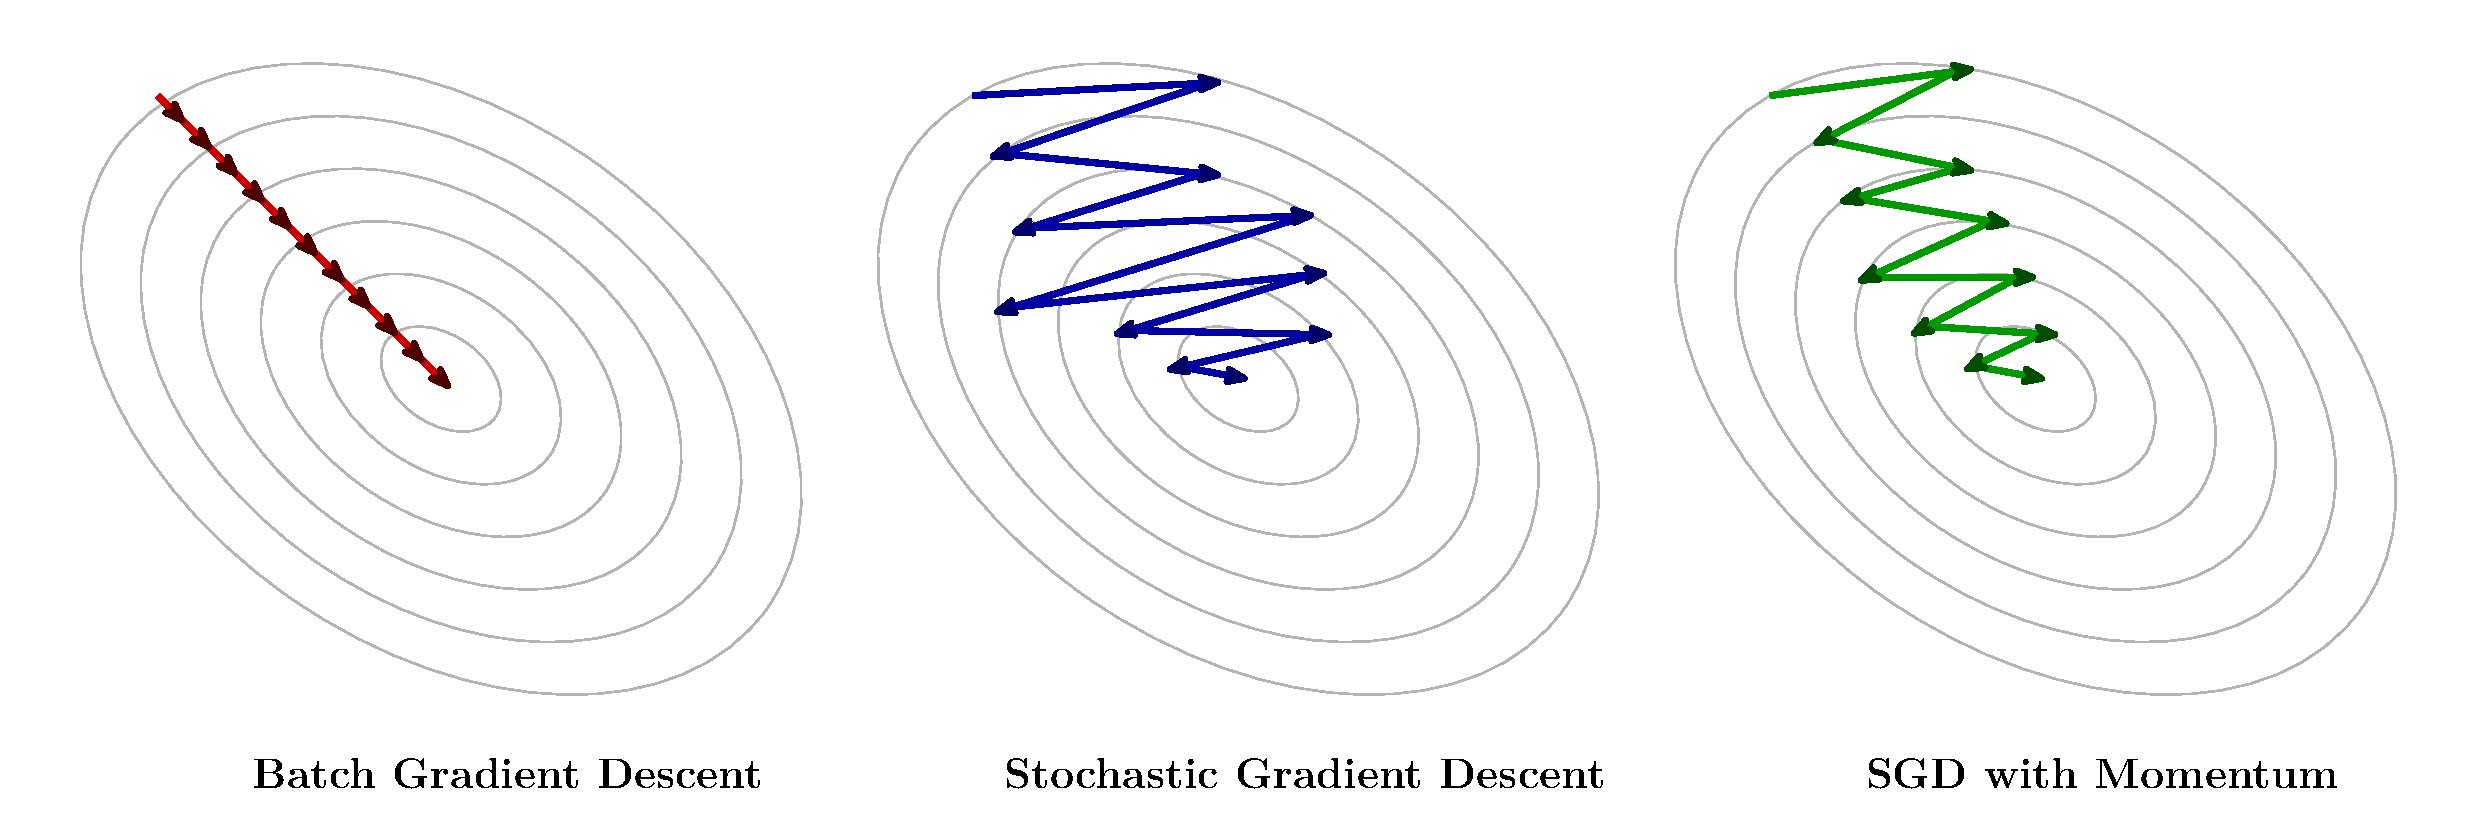
\includegraphics[width=\textwidth]{tikz/chapter3 - BGD vs SGD vs SGD with Momentum.pdf}
\caption{BGD vs SGD vs SGD with Momentum}
\end{figure}

\subsection{Stochastic Gradient Descent with Nesterov Momentum}

Stochastic Gradient Descent with Nesterov Momentum is a variant of the previous algorithm that adds a correction to the previous momentum before calculating the gradient. It works by firstly taking a step in the direction of the accumulated gradient (point 2 of the algorithm), and secondly calculating the gradient (point 4) and making the correction accordingly (point 5). (in simple momentum, we first compute the gradient and then make the correction) 

\begin{algorithm}
\renewcommand\thealgorithm{}
\caption{\textbf{\textcolor{mygreen}{Stochastic Gradient Descent with Nesterov Momentum}}}
\begin{algorithmic}[1]
\REQUIRE{Learning Rate $\varepsilon$}
\REQUIRE{Momentum Parameter $\alpha$}
\REQUIRE{Initial Parameters $\mathbf{w}$}
\REQUIRE{Initial Velocity $\mathbf{v}$}
\WHILE{Stopping Criteria not met}
\STATE Update parameters temporarily:
$\textcolor{mybluee}{\widetilde{\mathbf{w}} \leftarrow \mathbf{w} + \alpha \mathbf{v}}$
\STATE Compute gradient estimate on \textbf{\textcolor{myred}{a random training example}} $(\mathbf{x}^{(i)}, y^{(i)})$
\STATE $\mathbf{\hat{g}} \leftarrow \nabla_{\textcolor{mybluee}{\widetilde{\mathbf{w}}}} L(f(\mathbf{x}^{(i)},\textcolor{mybluee}{\widetilde{\mathbf{w}}}), y^{(i)})$
\STATE Update velocity:
$\textcolor{mybluee}{\mathbf{v} \leftarrow \alpha \mathbf{v} - \varepsilon \mathbf{\hat{g}}}$
\STATE Update parameters:
$\textcolor{mybluee}{\mathbf{w} \leftarrow \mathbf{w} + \mathbf{v}}$
\ENDWHILE
\end{algorithmic}
\end{algorithm}

The main difference between the Nesterov momentum and the standard momentum lies in \textbf{where the gradient is evaluated}. In the Nesterov momentum the gradient term is not calculated from the current position in parameter space, but rather from an intermediate position. This approach offers a significant advantage: while the gradient term always points in the optimal direction, \textbf{the momentum term may not align consistently}. Consequently, if the momentum goes in the wrong direction or overshoots the target, the gradient term can still "go back" and correct it \textbf{in the same update step}.

\newpage
\subsection{Adagrad (Adaptive Gradient Algorithm)}
The previous techniques that we have seen are based on the intuition of adjusting the learning rate while considering the history of past progress.

However, in many machine learning situations, we are faced with two distinct scenarios: a simpler one, in which all features are equally important, and a more difficult one, in which features have different levels of importance. However, up to this point, we have assigned the same learning rate to all features. \textit{Is this a valid idea?}

\begin{figure}[htbp]
\centering
\includegraphics[width=0.8\textwidth]{tikz/chapter3 - Features Importance.pdf}
\caption{Adaptive Learning Methods Intuition}
\end{figure}

Adagrad is an optimisation algorithm that \textbf{scales the model parameters by the square root of the sum of the squares of all historical gradient values}. This approach makes it possible to automatically adapt the learning rate for each parameter according to its update rate (in simple words, we take into account how much progress we have already done along each dimension and adjust the learning rate accordingly). 
\begin{algorithm}
\renewcommand\thealgorithm{}
\caption{\textbf{\textcolor{mygreen}{Adagrad}}}
\begin{algorithmic}[1]
\REQUIRE{Learning Rate $\varepsilon$}
\REQUIRE{Initial Parameters $\mathbf{w}$}
\REQUIRE{Small Constant $\delta$ to avoid division by zero}
\STATE Initialize sum of squared gradients vector: $\mathbf{r} \leftarrow 0$
\WHILE{Stopping Criteria not met}
\STATE Compute gradient estimate on \textbf{\textcolor{myred}{a random training example}} $(\mathbf{x}^{(i)}, y^{(i)})$
\STATE $\mathbf{\hat{g}} \leftarrow \nabla_{\mathbf{w}} L(f(\mathbf{x}^{(i)},\mathbf{w}), y^{(i)})$
\STATE Accumulate:
$\textcolor{mybluee}{\mathbf{r} \leftarrow \mathbf{r} + \mathbf{\hat{g}} \odot \mathbf{\hat{g}}}$
\STATE Update parameters:
$\textcolor{mybluee}{\mathbf{w} \leftarrow \mathbf{w} - \frac{\varepsilon}{\delta + \sqrt{\mathbf{r}}} \odot \mathbf{\hat{g}}}$ 
\ENDWHILE
\end{algorithmic}
\end{algorithm}

Where $\odot$ denotes element-wise multiplication.

Parameters that have large partial derivatives with respect to loss will see their learning rates reduced quickly, while those with smaller gradients will have higher learning rates, allowing for a \textbf{more stable convergence} of the model as not all direction of the optimization surface will have the same importance. 

\subsection{RMSProp (Root Mean Square Propagation)}

In many optimisation situations, Adagrad can excessively decrease the learning rate, making convergence difficult, especially in non-convex contexts. This occurs because Adagrad tends to aggressively adapt the learning rate according to the frequency of parameter updates. This means that if a parameter has a large variation in gradients during training (i.e. steep surface along that dimension), Adagrad will drastically reduce the learning rate for that parameter.

To address this problem, RMSProp has been proposed as a variant of Adagrad that \textbf{maintains an exponentially decreasing average of past gradients} (similar to momentum $\alpha v -\epsilon\hat{g}$), also called Running Average.

\begin{algorithm}
\renewcommand\thealgorithm{}
\caption{\textbf{\textcolor{mygreen}{RMSProp}}}
\begin{algorithmic}[1]
\REQUIRE{Learning Rate $\varepsilon$}
\REQUIRE{Decay Rate $\rho$}
\REQUIRE{Small constant $\delta$ to avoid division by zero}
\REQUIRE{Initial Parameters $\mathbf{w}$}
\STATE Initialize running average: $\mathbf{r} \leftarrow 0$
\WHILE{Stopping Criteria not met}
\STATE Compute gradient estimate on \textbf{\textcolor{myred}{a random training example}} $(\mathbf{x}^{(i)}, y^{(i)})$
\STATE $\mathbf{\hat{g}} \leftarrow \nabla_{\mathbf{w}} L(f(\mathbf{x}^{(i)},\mathbf{w}), y^{(i)})$
\STATE Accumulate:
$\textcolor{mybluee}{\mathbf{r} \leftarrow \rho \mathbf{r} + (1 - \rho) \mathbf{\hat{g}} \odot \mathbf{\hat{g}}}$
\STATE Update the parameters:
$\textcolor{mybluee}{\mathbf{w} \leftarrow \mathbf{w} - \frac{\varepsilon}{\delta + \sqrt{\mathbf{r}}} \odot \mathbf{\hat{g}}}$
\ENDWHILE
\end{algorithmic}
\end{algorithm}

Thanks to this strategy, RMSProp \textbf{avoids an excessive decrease in the learning rate}, as past gradients $r$ (that have been accumulated) counts less, and allows it to adapt better in non-convex contexts and to maintain a more stable convergence during optimisation. It is important to note that there is also a version of RMSProp that includes the Nesterov term, known as \textbf{RMSProp with Nesterov Momentum}, which can further improve the performance of the algorithm in certain situations.


\subsection{ADAM (ADAptive Moments)}
Adam is an optimisation algorithm that combines concepts derived from RMSProp and Momentum.  However, Adam introduces a fundamental innovation: \textbf{bias correction terms} for first and second moments. These terms are crucial since the first and second moments are initialised at zero and require time to "warm up" (i.e. to adapt to the data).

Adam automatically adapts the learning rates for each parameter based on momentum and past momentum estimation, helping to improve the effectiveness of optimisation during the learning process. In Adam, we combine several concepts seen in this section: the \textbf{use of the stochastic} in the SGD, the \textbf{idea of using momentum}, the \textbf{adaptation of the learning rate based on the second moment} and the \textbf{use of a bias correction} for both moments.
\newpage
\begin{algorithm}
\renewcommand\thealgorithm{}
\caption{\textbf{\textcolor{mygreen}{Adam}}}
\begin{algorithmic}[1]
\REQUIRE{Learning Rate $\varepsilon$}
\REQUIRE{Decay Rates for First and Second Moments $\rho_1$, $\rho_2$}
\REQUIRE{Small constant $\delta$ to avoid division by zero}
\REQUIRE{Initial Parameters $\mathbf{w}$}
\STATE Initialize first and second moments: $\mathbf{s} \leftarrow 0$, $\mathbf{r} \leftarrow 0$
\STATE Initialize time step $t \leftarrow 0$
\WHILE{Stopping Criteria not met}
\STATE Compute gradient estimate on \textbf{\textcolor{myred}{a random training example}} $(\mathbf{x}^{(i)}, y^{(i)})$
\STATE Compute the gradient: $\mathbf{\hat{g}} \leftarrow \nabla_{\mathbf{w}} L(f(\mathbf{x}^{(i)},\mathbf{w}), y^{(i)})$
\STATE Update time step: $t \leftarrow t + 1$
\STATE Update \textbf{biased} first moment estimate:
$\mathbf{s} \leftarrow \rho_1 \mathbf{s} + (1 - \rho_1) \mathbf{\hat{g}}$ \qquad \quad \qquad \COMMENT{\textbf{\textcolor{gray!90!white}{Momentum Idea}}}
\STATE Update \textbf{biased} second moment estimate:
$\mathbf{r} \leftarrow \rho_2 \mathbf{r} + (1 - \rho_2) \mathbf{\hat{g}} \odot \mathbf{\hat{g}}$ \qquad \COMMENT{\textbf{\textcolor{gray!90!white}{RMSProp Idea}}}
\STATE Correct bias in first moment: $\textcolor{mybluee}{\hat{\mathbf{s}} \leftarrow \frac{\mathbf{s}}{1 - \rho_1^t}}$
\STATE Correct bias in second moment: $\textcolor{mybluee}{\hat{\mathbf{r}} \leftarrow \frac{\mathbf{r}}{1 - \rho_2^t}}$
\STATE Update parameters:
$\textcolor{mybluee}{\mathbf{w} \leftarrow \mathbf{w} - \varepsilon \frac{\hat{\mathbf{s}}}{\delta + \sqrt{\hat{\mathbf{r}}}}}$
\ENDWHILE
\end{algorithmic}
\end{algorithm}

\vspace{-0.5cm}
\section{Normalization}

\vspace{-0.4cm}
In the world of neural networks, optimization is crucial to model success. However, simply adopting SGD may not be enough. Deep neural networks are known to be difficult to train, for example, one of the main problems we face during optimization is the so-called "Covariate Shift."
\vspace{-0.4cm}

\subsection{The Problem of Covariate Shift}

When training a neural network, it is important to keep the distribution of input data stable throughout the training process. If the distribution changes significantly during training, the model may have difficulty generalizing well to new data, as patterns learned during training may no longer be relevant or representative.

The main problem arising from the covariate shift is that it can lead to a situation where \textbf{most of the input data falls into non-linear regions} of the neural network's activation function. This can significantly \textbf{slow down the learning process} as the network may require multiple iterations to adapt its weights effectively to the new input distributions.

To address the Covariate Shift problem and improve the training of neural networks, a fundamental concept was introduced: \textbf{Batch Normalization}.

\subsection{Batch Normalization}

It is a method for reconfiguring the parameters of a deep network, which \textbf{can be applied to the input layer as well as to any hidden layer}.

The key concept behind Batch Normalization is the standardization of the inputs of a network layer. This is done by subtracting the mean of the inputs and dividing by the standard deviation. In mathematical terms, if $ \mathbf{H} $ represents the outputs of a layer, $ \mu $ and $ \sigma $ represent the mean and standard deviation (both vectors) calculated on the columns (features) of $ \mathbf{H} $, then the transformation is given by:
$$ \mathbf{H}' = \frac{\mathbf{H} - \mu}{\sigma} $$ where $$\mu = \frac{1}{m}\sum_{}^{j}\mathbf{H}_{:,j}$$
$$\sigma = \sqrt{\delta + \frac{1}{m}\sum_{j}^{}(\mathbf{H}-\mu)^2_j}$$
\textit{The term $\delta$ in the formula represents the usual small constant added to avoid numerical problems when the calculated standard deviation is very close to zero. }
Standardizing the output of a unit could limit the expressive power of the neural network because, without introducing additional parameters, normalization could bring all features in a given stratum to a common scale, making it more difficult for the neural network to capture complexity and variation in the data. This is because standardization unifies features, bringing them to \textbf{a mean of zero and a standard deviation of one}, potentially "squeezing" them into a narrower range.

To mitigate this problem and allow the neural network to maintain its expressive capability, two additional parameters are introduced in Batch Normalization: the \textbf{scaling factor} ($ \gamma $) and the \textbf{bias} ($ \beta $). These parameters allow the network to learn a linear transformation of the normalized output, thus allowing greater flexibility in data representation. 
$$\text{Output} = \gamma \mathbf{H}' + \beta $$
Essentially, the scaling factor and bias allow the network to adapt to a wide range of data while maintaining its ability to express and learn complex patterns as they are learned during the back-propagation process.

During training, back-propagation is performed through normalized activations and these two parameters ($\gamma$ and $\beta$) are also learned. During testing, on the other hand, running averages of $ \mu $ and $ \sigma $ collected during training are used to evaluate new entries.

% Batch Normalization offers several advantages, including improving gradient flow, enabling the use of higher learning rates, reducing dependence on initial parameters, and functioning as a form of regularization to improve stability and prevent overfitting during neural network training.

\subsection{Batch, Layer or Instance Normalization?}

There are two famous variants of Batch Normalization: \textbf{Layer Normalization} and \textbf{Instance Normalization}. Briefly summarised, the difference is that Batch Normalization normalises across the entire batch, Layer Normalization normalises across the entire layer and Instance Normalization normalises each instance individually. \textit{I know, it's not very intuitive, so let's do a more detailed analysis!}

To explain the various concepts, we will use a tuple \textbf{(N,C,H,W)}, which is commonly used to represent multidimensional data such as images (\textit{which will be the focus of our example to give us a better understanding}). This representation is nothing more than a tensor and is common in frameworks such as TensorFlow and PyTorch to handle input data in neural networks. Here is what each dimension represents:
\begin{itemize}
    \item \textbf{N}: Represents the \textbf{batch size}, i.e. the number of instances (or samples) within the batch. For example, if N=32, this means we are working with a batch of 32 images.
    \item \textbf{C}: Indicates the \textbf{number of channels} (feature maps) in the data. In a color image, we will typically have 3 channels for the colors red, green and blue (RGB). In general, in the input data, the channel can represent not only the color, but various aspects or features of the input, such as depth, features extracted from convolutional layers, etc.
    \item \textbf{H}: Represents the \textbf{height of the data}. In an image, it corresponds to the number of rows of pixels present.
    \item \textbf{W}: Represents the \textbf{width of the data}. In an image, it corresponds to the number of columns of pixels present.
\end{itemize}
H and W will be merged together (\textit{Sorry, but my drawing skills stop at 3 dimensions \faSadTear[regular]}).
We will also use a small example: let us consider a batch with 10 images, each of which has 3 features (RGB) and the image size is 100x100. Let's start then:


\begin{minipage}{0.4\textwidth}
\textbf{\textcolor{mybluee!70}{Batch Normalization (BN):}} \\

Consider the entire batch of size N. Each example in the batch has C channels, each of which has an image of size HxW. With Batch Normalization, we normalise the data on each channel across the entire batch. Then, for each channel, we calculate the mean and standard deviation over all examples in the batch and normalise the data on that channel accordingly.
\end{minipage}
\begin{minipage}{0.05\textwidth}
\ 
\end{minipage}
\begin{minipage}{0.55\textwidth}
\includegraphics[width=\textwidth]{tikz/chapter3 - Batch Norm.pdf}
\captionof{figure}{Batch Norm Multidimensional Data}
\end{minipage}

Taking our example, we would have a tensor of size (10, 3, 100), where:
10 represents the batch size (N), i.e. the number of images in the batch,
3 represents the number of channels (C), such as the three color channels: red, green and blue,
100 represents the height (H) of the image and
100 represents the width (W) of the image.
For each color channel in each image, the mean and standard deviation on all pixels corresponding to that color channel in all images in the batch would be calculated. The pixel values for each color channel \textbf{in each image} would then be normalised against these calculated mean and standard deviations.



\begin{minipage}{0.55\textwidth}
\includegraphics[width=\textwidth]{tikz/chapter3 - Layer Norm.pdf}
\captionof{figure}{Layer Norm Multidimensional Data}
\end{minipage}
\begin{minipage}{0.05\textwidth}
\ 
\end{minipage}
\begin{minipage}{0.4\textwidth}
\textbf{\textcolor{myred!70}{Layer Normalization (LN):}} \\

Here, we consider each example in the batch separately. Each example has C channels (features!), each of which has an image of size HxW. With Layer Normalization, we normalise the data of each channel for each example. Then, for each channel, we calculate the mean and standard deviation over the entire input of that example (i.e. over all positions of HxW) and normalise the data of that channel accordingly.
\end{minipage}

Once again, we would have a tensor of size (10, 3, 100).
However, each image in the batch is considered separately. For each image, the pixel values in each color channel would be normalised with respect to the distribution of pixel values within the same image.
Thus, the pixel values in each image would be normalised to the distribution of pixel values within the image itself, \textbf{completely ignoring the other images in the batch}.


\begin{minipage}{0.4\textwidth}
\textbf{\textcolor{mygreen!70}{Instance Normalization (IN):}} \\

We consider each spatial position (HxW) separately for each example in the batch. Each position has C channels. With Instance Normalization, we normalise the data of each channel for each position in the image. Then, for each channel, we calculate the mean and standard deviation over all positions in the image for each example in the batch and normalise the data for that channel accordingly.
\end{minipage}
\begin{minipage}{0.05\textwidth}
\ 
\end{minipage}
\begin{minipage}{0.55\textwidth}
\includegraphics[width=\textwidth]{tikz/chapter3 - Instance Norm.pdf}
\captionof{figure}{Instance Norm Multidimensional Data}
\end{minipage}

Here again, we have the same size tensor (10, 3, 100).
Now, each pixel in each color channel of each spatial position in the image is considered separately for each image in the batch.
The pixel values at each spatial position (HxW) of \textbf{each color channel in each image} would be normalised to the corresponding pixel values at the same positions in the other images in the batch.

\textbf{N.B.} A more modern technique is \textbf{Group Normalisation (GN)}, which can be considered as a mix between Layer Normalisation and Instance Normalisation. With GN, the data channels are considered separately, as in Layer Normalisation, but instead of operating on an entire layer, the \textbf{channels are divided into groups} and the normalisation statistics within each group are calculated independently. This approach is reminiscent of the idea of instance-based normalisation, where each instance is considered separately, but instead of normalising individual instances, GN normalises groups of channels. This makes it useful in scenarios where the dimensionality of the data is high and normalisation on entire layers may be excessive.


